\documentclass{article}
\usepackage{graphicx}
\usepackage[utf8]{inputenc}
\usepackage[T1]{fontenc}
\usepackage{fouriernc}
\usepackage[margin=1in]{geometry}
\usepackage{amsmath}
\begin{document}

\begin{titlepage}
	\centering 
	\scshape
	\vspace*{\baselineskip}
	\rule{\textwidth}{1.6pt}\vspace*{-\baselineskip}\vspace*{2pt}
	\rule{\textwidth}{0.4pt} 
	\vspace{0.75\baselineskip}
	
	{\Large CS 374 : Computational and Numerical Methods \\\vspace{0.75\baselineskip} Set 4}
	\vspace{0.75\baselineskip}
	
	\rule{\textwidth}{0.4pt}\vspace*{-\baselineskip}\vspace{3.2pt} 
	\rule{\textwidth}{1.6pt}
	
	\vspace{2\baselineskip}  
	The Bisection Method
	
	\vspace*{3\baselineskip}
	
	\vspace{0.5\baselineskip} %originally 0.5
	
	{\scshape\large Purvil Mehta (201701073) \\ Bhargey Mehta (201701074) \\} 
	
	\vspace{1\baselineskip} 
	
	\textit{Dhirubhai Ambani Institute of Information and Communication Technology \\ Gandhinagar\\} 
	\vspace*{2\baselineskip}
	\today


\end{titlepage}


\newpage
\tableofcontents
\newpage

\section{$f(x)$ = $x^6 - x - 1$}

\subsection{Plots}
\begin{figure}[!h]
    \centering
    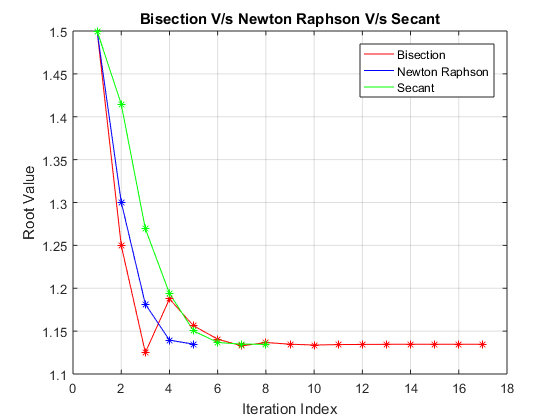
\includegraphics[scale=0.55]{1_1.png}
    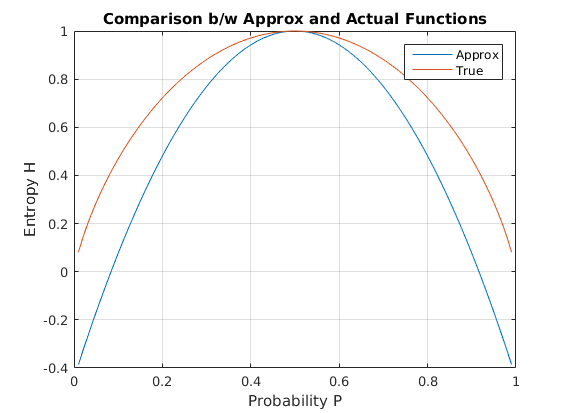
\includegraphics[scale=0.55]{1_2.png}
    \caption{Fig 1.1 : Positive root of $x^6 - x -1 = 0$ 
     || Fig 1.2: Negative root of $x^6 - x -1 = 0$}
\end{figure}

\subsection{Tables}
\begin{table}[!h]
\centering{\Large
\begin{tabular}{|c|c|c|c|c|c|}\hline
ItrNo   & $x_n$    & $f(x_n)$      & $f'(x_n)$      & $x_{n+1}$    & $x_{n+1}-x_n$ \\ \hline
1 & 1.5    & 8.8906 & 44.563 & 1.3005 & -0.1995   \\
2 & 1.3005 & 2.5373 & 21.32  & 1.1815 & -0.119    \\
3 & 1.1815 & 0.5385 & 12.813 & 1.1395 & -0.042    \\
4 & 1.1395 & 0.0492 & 10.525 & 1.1348 & -0.0047   \\
5 & 1.1348 & 0.0006 & 10.29  & 1.1347 & -0.0001   \\
\hline
\end{tabular}}
\caption{Positive Root of $x^6 - x - 1 =0$}
\end{table}
\begin{table}[!h]
\centering{\Large
\begin{tabular}{|c|c|c|c|c|c|}\hline
ItrNo   & $x_n$    & $f(x_n)$      & $f'(x_n)$      & $x_{n+1}$    & $x_{n+1}-x_n$ \\ \hline
1 & -1      & 1      & -7      & -0.8571 & 0.1429 \\
2 & -0.8571 & 0.2537 & -3.776  & -0.79   & 0.0672 \\
3 & -0.79   & 0.033  & -2.8457 & -0.7784 & 0.0116 \\
4 & -0.7784 & 0.0008 & -2.7143 & -0.7781 & 0.0003 \\
5 & -0.7781 & 0      & -2.7112 & -0.7781 & 0  \\
\hline
\end{tabular}}
\caption{Positive Root of $x^6 - x - 1 =0$}
\end{table}



\newpage
\section{$f(x)$ = $x^3 - x^2 - x - 1$}
\subsection{Plots}
\begin{figure}[!h]
    \centering
    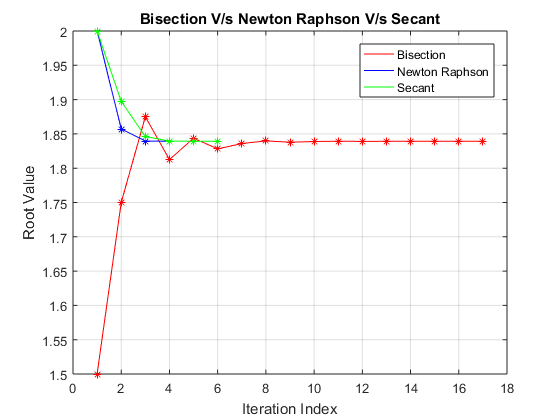
\includegraphics[scale=0.8]{2.png}
    \caption{Positive root of $x^3 - x^2 x -1 = 0$ }
\end{figure}
\subsection{Tables}
\begin{table}[!h]
\centering{\Large
\begin{tabular}{|c|c|c|c|c|c|}\hline
ItrNo   & $x_n$    & $f(x_n)$      & $f'(x_n)$      & $x_{n+1}$    & $x_{n+1}-x_n$ \\ \hline
1 & 2      & 1      & 7      & 1.8571 & -0.1429 \\
2 & 1.8571 & 0.0991 & 5.6327 & 1.8395 & -0.0176 \\
3 & 1.8395 & 0.0014 & 5.4727 & 1.8393 & -0.0003 \\
4 & 1.8393 & 0      & 5.4704 & 1.8393 & 0       \\
\hline
\end{tabular}}
\caption{Positive Root of $f(x)$ = $x^3 - x^2 - x - 1$}
\end{table}



\newpage
\section{$f(x) = 1 +0.3cos(x) - x$}
\subsection{Plots}
\begin{figure}[!h]
    \centering
    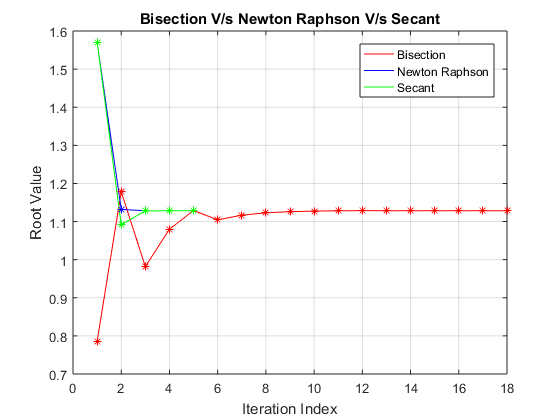
\includegraphics[scale=0.8]{3.png}
    \caption{Positive root of $1 + 0.3\cos{x} - x$ }
\end{figure}
\subsection{Tables}
\begin{table}[!h]
\centering{\Large
\begin{tabular}{|c|c|c|c|c|c|}\hline
ItrNo   & $x_n$    & $f(x_n)$      & $f'(x_n)$      & $x_{n+1}$    & $x_{n+1}-x_n$ \\ \hline
1 & 1.5708 & -0.5708 & -1.3    & 1.1317 & -0.4391 \\
2 & 1.1317 & -0.0042 & -1.2715 & 1.1284 & -0.0033 \\
3 & 1.1284 & 0       & -1.2711 & 1.1284 & 0       \\
\hline
\end{tabular}}
\caption{Positive Root of $f(x) = 1 +0.3cos(x) - x$}
\end{table}

\newpage
\section{$f(x) = 0.5 + \sin{x} - \cos{x}$}
\subsection{Plots}
\begin{figure}[!h]
    \centering
    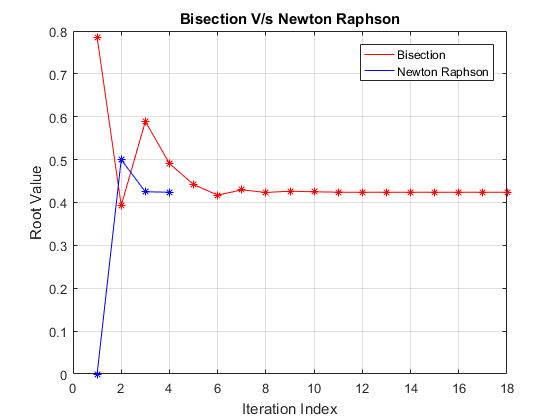
\includegraphics[scale=0.8]{4.png}
    \caption{Positive root of $f(x) = 0.5 + \sin{x} - \cos{x}$ }
\end{figure}
\subsection{Tables}
\begin{table}[!h]
\centering{\Large
\begin{tabular}{|c|c|c|c|c|c|}\hline
ItrNo   & $x_n$    & $f(x_n)$      & $f'(x_n)$      & $x_{n+1}$    & $x_{n+1}-x_n$ \\ \hline
1 & 0     & -0.5   & 1      & 0.5   & 0.5     \\
2 & 0.5   & 0.1018 & 1.357  & 0.425 & -0.075  \\
3 & 0.425 & 0.0012 & 1.3233 & 0.424 & -0.0009 \\
4 & 0.424 & 0      & 1.3229 & 0.424 & 0       \\
\hline
\end{tabular}}
\caption{Positive Root of $f(x) = 0.5 + \sin{x} - \cos{x}$}
\end{table}


\newpage
\section{$f(x) = x - e^{-x}$}
\subsection{Plots}
\begin{figure}[!h]
    \centering
    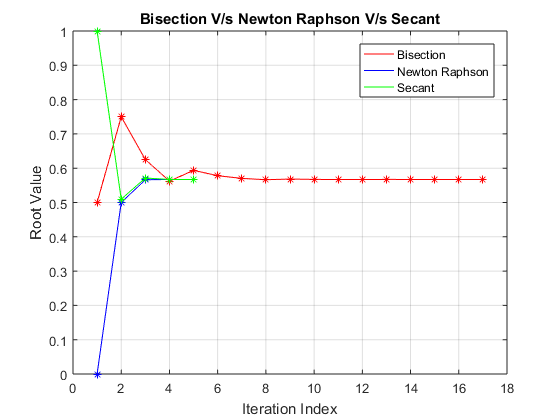
\includegraphics[scale=0.8]{5.png}
    \caption{Positive root of $f(x) = x - e^{-x}$ }
\end{figure}
\subsection{Tables}
\begin{table}[!h]
\centering{\Large
\begin{tabular}{|c|c|c|c|c|c|}\hline
ItrNo   & $x_n$    & $f(x_n)$      & $f'(x_n)$      & $x_{n+1}$    & $x_{n+1}-x_n$ \\ \hline
1 & 0      & 1      & -2      & 0.5    & 0.5    \\
2 & 0.5    & 0.1065 & -1.6065 & 0.5663 & 0.0663 \\
3 & 0.5663 & 0.0013 & -1.5676 & 0.5671 & 0.0008 \\
4 & 0.5671 & 0      & -1.5671 & 0.5671 & 0      \\
\hline
\end{tabular}}
\caption{Positive Root of $f(x) = x - e^{-x}$}
\end{table}


\newpage
\section{$f(x) = \sin{x} - e^{-x}$}
\subsection{Plots}
\begin{figure}[!h]
    \centering
    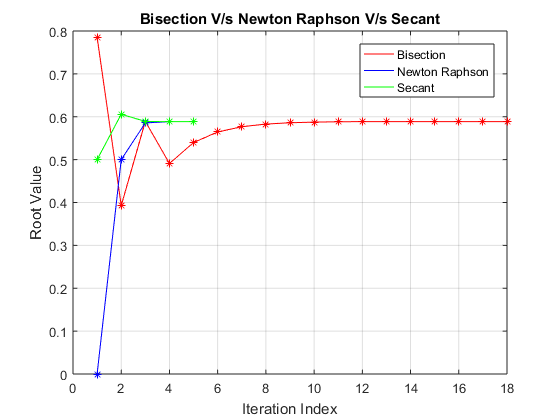
\includegraphics[scale=0.55]{6_1.png}
    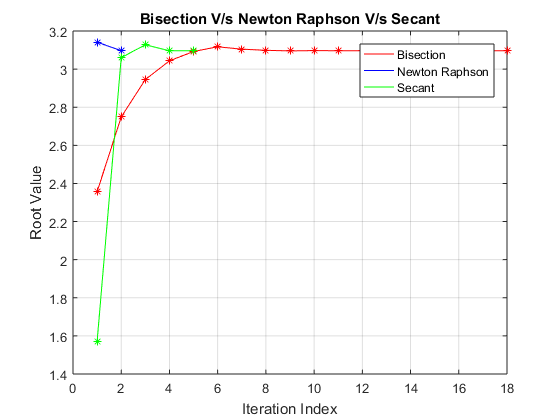
\includegraphics[scale=0.55]{6_2.png}
    \caption{Fig 1.1 : Positive root of $x^6 - x -1 = 0$ 
     || Fig 1.2: Negative root of $x^6 - x -1 = 0$}
\end{figure}
\subsection{Tables}
\begin{table}[!h]
\centering{\Large
\begin{tabular}{|c|c|c|c|c|c|}\hline
ItrNo   & $x_n$    & $f(x_n)$      & $f'(x_n)$      & $x_{n+1}$    & $x_{n+1}-x_n$ \\ \hline
1 & 0      & 1      & -2      & 0.5    & 0.5    \\
2 & 0.5    & 0.1271 & -1.4841 & 0.5856 & 0.0856 \\
3 & 0.5856 & 0.004  & -1.3901 & 0.5885 & 0.0029 \\
4 & 0.5885 & 0      & -1.3869 & 0.5885 & 0      \\
\hline
\end{tabular}}
\caption{Positive Root of $f(x) = \sin{x} - e^{-x}$}
\end{table}
\begin{table}[!h]
\centering{\Large
\begin{tabular}{|c|c|c|c|c|c|}\hline
ItrNo   & $x_n$    & $f(x_n)$      & $f'(x_n)$      & $x_{n+1}$    & $x_{n+1}-x_n$ \\ \hline
1 & 3.1416 & 0.0432 & 0.9568 & 3.0964 & -0.0452 \\
2 & 3.0964 & 0.0001 & 0.9538 & 3.0964 & -0.0001 \\
\hline
\end{tabular}}
\caption{Positive Root of $f(x) = \sin{x} - e^{-x}$}
\end{table}



\newpage
\section{$f(x) = x^3 -2x -2$}
\subsection{Plots}
\begin{figure}[!h]
    \centering
    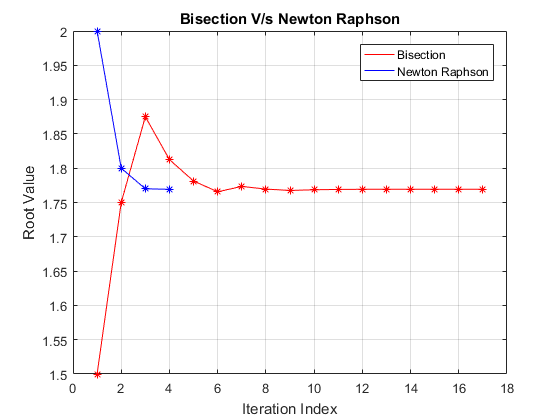
\includegraphics[scale=0.8]{7.png}
    \caption{Positive root of $x^3 -2x - 2= 0$}
\end{figure}
\subsection{Tables}
\begin{table}[!h]
\centering{\Large
\begin{tabular}{|c|c|c|c|c|c|}\hline
ItrNo   & $x_n$    & $f(x_n)$      & $f'(x_n)$      & $x_{n+1}$    & $x_{n+1}-x_n$ \\ \hline
1 & 2      & 2      & 10     & 1.8    & -0.2    \\
2 & 1.8    & 0.232  & 7.72   & 1.7699 & -0.0301 \\
3 & 1.7699 & 0.0048 & 7.3981 & 1.7693 & -0.0007 \\
4 & 1.7693 & 0      & 7.3912 & 1.7693 & 0       \\
\hline
\end{tabular}}
\caption{Positive Root of $f(x) = x^3 -2x -2$}
\end{table}



\newpage
\section{$f(x) = x^4 -x -1$}
\subsection{Plots}
\begin{figure}[!h]
    \centering
    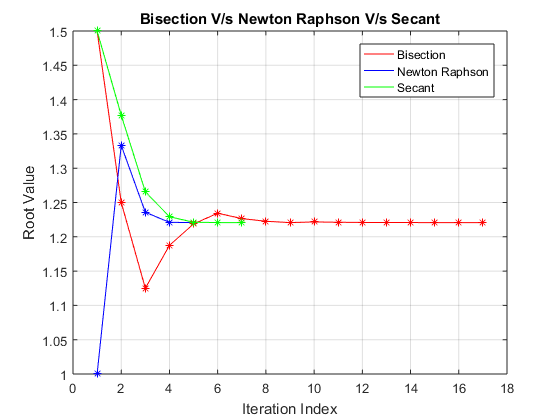
\includegraphics[scale=0.55]{8_1.png}
    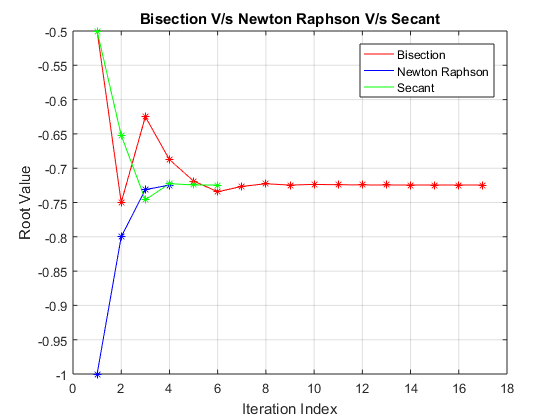
\includegraphics[scale=0.55]{8_2.png}
    \caption{Roots of $x^4 -x - 1= 0$}
\end{figure}
\subsection{Tables}
\begin{table}[!h]
\centering{\Large
\begin{tabular}{|c|c|c|c|c|c|}\hline
ItrNo   & $x_n$    & $f(x_n)$      & $f'(x_n)$      & $x_{n+1}$    & $x_{n+1}-x_n$ \\ \hline
1 & 1      & -1     & 3      & 1.3333 & 0.3333  \\
2 & 1.3333 & 0.8272 & 8.4815 & 1.2358 & -0.0975 \\
3 & 1.2358 & 0.0966 & 6.5494 & 1.2211 & -0.0147 \\
4 & 1.2211 & 0.002  & 6.2823 & 1.2207 & -0.0003 \\
5 & 1.2207 & 0      & 6.2767 & 1.2207 & 0  \\
\hline
\end{tabular}}
\caption{First Root of $f(x) = x^4 -x -1$}
\end{table}

\begin{table}[!h]
\centering{\Large
\begin{tabular}{|c|c|c|c|c|c|}\hline
ItrNo   & $x_n$    & $f(x_n)$      & $f'(x_n)$      & $x_{n+1}$    & $x_{n+1}-x_n$ \\ \hline
1 & -1      & 1      & -5      & -0.8    & 0.2    \\
2 & -0.8    & 0.2096 & -3.048  & -0.7312 & 0.0688 \\
3 & -0.7312 & 0.0171 & -2.564  & -0.7245 & 0.0067 \\
4 & -0.7245 & 0.0001 & -2.5215 & -0.7245 & 0.0001 \\
\hline
\end{tabular}}
\caption{Second Root of $f(x) = x^4 -x -1$}
\end{table}



\newpage
\section{$f(x) = e^x -x -2$}
\subsection{Plots}
\begin{figure}[!h]
    \centering
    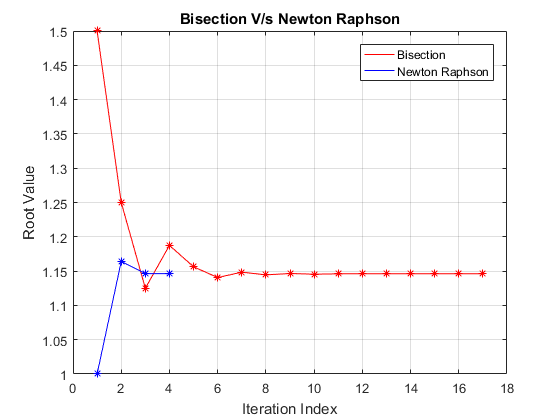
\includegraphics[scale=0.8]{9.png}
    \caption{Positive root of $f(x) = e^x -x -2$}
\end{figure}
\subsection{Tables}
\begin{table}[!h]
\centering{\Large
\begin{tabular}{|c|c|c|c|c|c|}\hline
ItrNo   & $x_n$    & $f(x_n)$      & $f'(x_n)$      & $x_{n+1}$    & $x_{n+1}-x_n$ \\ \hline
1 & 1      & -0.2817 & 1.7183 & 1.164  & 0.164   \\
2 & 1.164  & 0.0386  & 2.2026 & 1.1464 & -0.0175 \\
3 & 1.1464 & 0.0005  & 2.1469 & 1.1462 & -0.0002 \\
4 & 1.1462 & 0       & 2.1462 & 1.1462 & 0       \\
\hline
\end{tabular}}
\caption{Positive Root of $f(x) = e^x -x -2$}
\end{table}


\newpage
\section{$f(x) = 1 -x +\sin{x}$}
\subsection{Plots}
\begin{figure}[!h]
    \centering
    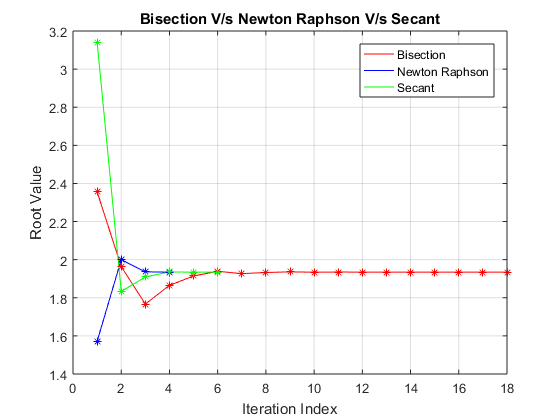
\includegraphics[scale=0.8]{10.png}
    \caption{Positive root of $f(x) = 1 -x +\sin{x}$}
\end{figure}
\subsection{Tables}
\begin{table}[!h]
\centering{\Large
\begin{tabular}{|c|c|c|c|c|c|}\hline
ItrNo   & $x_n$    & $f(x_n)$      & $f'(x_n)$      & $x_{n+1}$    & $x_{n+1}-x_n$ \\ \hline
1 & 1.5708 & 0.4292  & -1      & 2      & 0.4292  \\
2 & 2      & -0.0907 & -1.4161 & 1.936  & -0.064  \\
3 & 1.936  & -0.0019 & -1.3571 & 1.9346 & -0.0014 \\
4 & 1.9346 & 0       & -1.3558 & 1.9346 & 0       \\
\hline
\end{tabular}}
\caption{Positive Root of $f(x) = 1 -x +\sin{x}$}
\end{table}



\newpage
\section{$f(x) = -x +\tan{x}$}
\subsection{Plots}
\begin{figure}[!h]
    \centering
    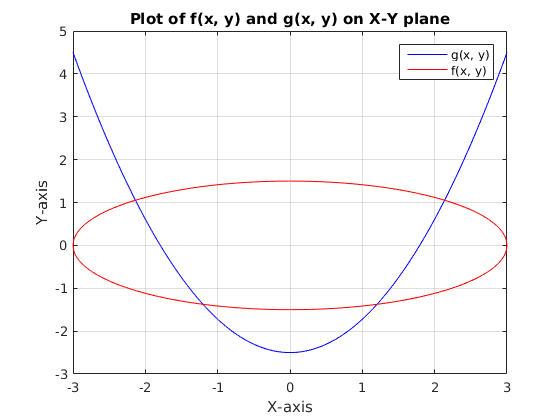
\includegraphics[scale=0.55]{11_1.png}
    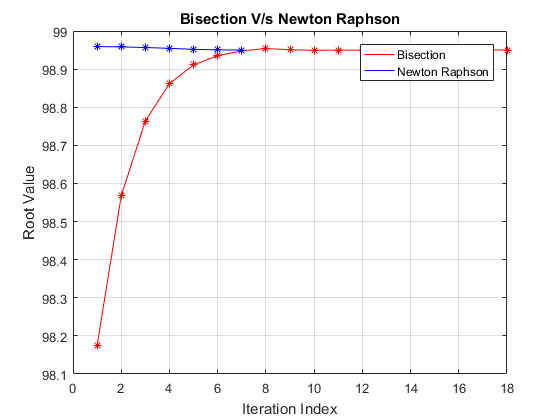
\includegraphics[scale=0.55]{11_2.png}
    \caption{Root of $f(x) = -x +\tan{x}$}
\end{figure}
\subsection{Tables}
\begin{table}[!h]
\centering{\Large
\begin{tabular}{|c|c|c|c|c|c|}\hline
ItrNo   & $x_n$    & $f(x_n)$      & $f'(x_n)$      & $x_{n+1}$    & $x_{n+1}-x_n$ \\ \hline
1 & 4.6124 & 5.3543 & 99.334 & 4.5585 & -0.0539 \\
2 & 4.5585 & 1.8878 & 41.554 & 4.5131 & -0.0454 \\
3 & 4.5131 & 0.4371 & 24.504 & 4.4952 & -0.0178 \\
4 & 4.4952 & 0.0369 & 20.54  & 4.4934 & -0.0018 \\
5 & 4.4934 & 0.0003 & 20.194 & 4.4934 & 0   \\   
\hline
\end{tabular}}
\caption{The first Root of $f(x) = -x +\tan{x}$}
\end{table}
\begin{table}[!h]
\centering{\Large
\begin{tabular}{|c|c|c|c|c|c|}\hline
ItrNo   & $x_n$    & $f(x_n)$      & $f'(x_n)$      & $x_{n+1}$    & $x_{n+1}-x_n$ \\ \hline
1 & 98.959 & 901.04 & 1000000     & 98.958 & -0.0009 \\
2 & 98.958 & 427.07 & 2767005 & 98.957 & -0.0015 \\
3 & 98.957 & 191.36 & 84286     & 98.954 & -0.0023 \\
4 & 98.954 & 76.026 & 30618     & 98.952 & -0.0025 \\
5 & 98.952 & 23.028 & 14879     & 98.95  & -0.0015 \\
6 & 98.95  & 3.6571 & 10528     & 98.95  & -0.0003 \\
7 & 98.95  & 0.1259 & 9816      & 98.95  & 0    \\
\hline
\end{tabular}}
\caption{The Root of $f(x) = -x +\tan{x}$ around 100}
\end{table}


\newpage
\section{$f(x) = ax(1-x)$}
\subsection{f(x) converging towards $x = 0$}
\subsubsection{Plots}
\begin{figure}[!h]
    \centering
    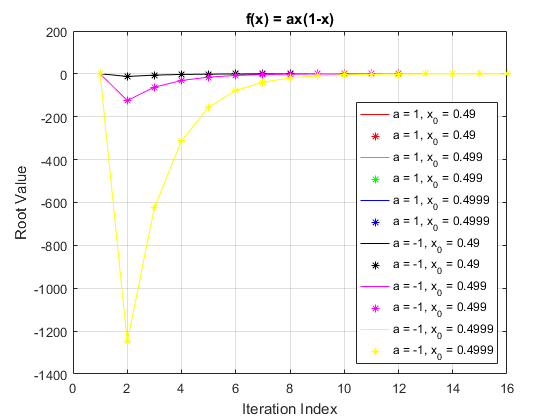
\includegraphics[scale=0.8]{q3.png}
    \caption{Positive root of $f(x) = ax(1-x)$}
\end{figure}
\subsubsection{Tables}
\begin{table}[!ht]
\centering{\Large
\begin{tabular}{|c|c|c|c|c|c|}\hline
ItrNo   & $x_n$    & $f(x_n)$      & $f'(x_n)$      & $x_{n+1}$    & $x_{n+1}-x_n$ \\ \hline
1 & 0.49    & 0.2499  & 0.02   & -12.005 & -12.495 \\
2 & -12.005 & -156.13 & 25.01  & -5.7625 & 6.2425  \\
3 & -5.7625 & -38.969 & 12.525 & -2.6512 & 3.1113  \\
4 & -2.6512 & -9.6801 & 6.3024 & -1.1153 & 1.5359  \\
5 & -1.1153 & -2.3591 & 3.2305 & -0.385  & 0.7302  \\
6 & -0.385  & -0.5333 & 1.77   & -0.0838 & 0.3013  \\
7 & -0.0838 & -0.0908 & 1.1675 & -0.006  & 0.0777  \\
8 & -0.006  & -0.006  & 1.012  & 0       & 0.006   \\
9 & 0       & 0       & 1.0001 & 0       & 0      \\
\hline
\end{tabular}}
\caption{Root of $f(x) = ax(1-x)$ where $a = 1$ and Initial Point = $0.49$}
\end{table}
\begin{table}[!ht]
\centering{\Large
\begin{tabular}{|c|c|c|c|c|c|}\hline
ItrNo   & $x_n$    & $f(x_n)$      & $f'(x_n)$      & $x_{n+1}$    & $x_{n+1}-x_n$ \\ \hline
1  & 0.499   & 0.25    & 0.002  & -124.5  & -125   \\
2  & -124.5  & -15625  & 250    & -62.001 & 62.499 \\
3  & -62.001 & -3906.2 & 125    & -30.753 & 31.249 \\
4  & -30.753 & -976.48 & 62.505 & -15.13  & 15.622 \\
5  & -15.13  & -244.06 & 31.261 & -7.3232 & 7.8072 \\
6  & -7.3232 & -60.952 & 15.646 & -3.4276 & 3.8956 \\
7  & -3.4276 & -15.176 & 7.8551 & -1.4956 & 1.932  \\
8  & -1.4956 & -3.7324 & 3.9912 & -0.5604 & 0.9352 \\
9  & -0.5604 & -0.8745 & 2.1209 & -0.1481 & 0.4123 \\
10 & -0.1481 & -0.17   & 1.2962 & -0.0169 & 0.1312 \\
11 & -0.0169 & -0.0172 & 1.0338 & -0.0003 & 0.0166 \\
12 & -0.0003 & -0.0003 & 1.0006 & 0       & 0.0003 \\
13 & 0       & 0       & 1      & 0       & 0 \\
\hline
\end{tabular}}
\caption{Root of $f(x) = ax(1-x)$ where $a = 1$ and Initial Point = $0.499$}
\end{table}
\newpage
\begin{table}[!ht]
\centering{\Large
\begin{tabular}{|c|c|c|c|c|c|}\hline
ItrNo   & $x_n$    & $f(x_n)$      & $f'(x_n)$      & $x_{n+1}$    & $x_{n+1}-x_n$ \\ \hline
1  & 0.4999  & 0.25        & 0.0002 & -1249.5 & -1250  \\
2  & -1249.5 & -1.5625e+06 & 2500   & -624.5  & 625    \\
3  & -624.5  & -3.9062e+05 & 1250   & -312    & 312.5  \\
4  & -312    & -97656      & 625    & -155.75 & 156.25 \\
5  & -155.75 & -24414      & 312.5  & -77.626 & 78.124 \\
6  & -77.626 & -6103.4     & 156.25 & -38.565 & 39.061 \\
7  & -38.565 & -1525.8     & 78.129 & -19.035 & 19.529 \\
8  & -19.035 & -381.39     & 39.071 & -9.2742 & 9.7614 \\
9  & -9.2742 & -95.284     & 19.548 & -4.3999 & 4.8743 \\
10 & -4.3999 & -23.759     & 9.7997 & -1.9754 & 2.4244 \\
11 & -1.9754 & -5.8778     & 4.9509 & -0.7882 & 1.1872 \\
12 & -0.7882 & -1.4095     & 2.5764 & -0.2411 & 0.5471 \\
13 & -0.2411 & -0.2993     & 1.4823 & -0.0392 & 0.2019 \\
14 & -0.0392 & -0.0408     & 1.0785 & -0.0014 & 0.0378 \\
15 & -0.0014 & -0.0014     & 1.0029 & 0       & 0.0014 \\
16 & 0       & 0           & 1      & 0       & 0   \\
\hline
\end{tabular}}
\caption{Root of $f(x) = ax(1-x)$ where $a = 1$ and Initial Point = $0.4999$}
\end{table}
\begin{table}[!ht]
\centering{\Large
\begin{tabular}{|c|c|c|c|c|c|}\hline
ItrNo   & $x_n$    & $f(x_n)$      & $f'(x_n)$      & $x_{n+1}$    & $x_{n+1}-x_n$ \\ \hline
1 & 0.49    & -0.2499 & -0.02   & -12.005 & -12.495 \\
2 & -12.005 & 156.13  & -25.01  & -5.7625 & 6.2425  \\
3 & -5.7625 & 38.969  & -12.525 & -2.6512 & 3.1113  \\
4 & -2.6512 & 9.6801  & -6.3024 & -1.1153 & 1.5359  \\
5 & -1.1153 & 2.3591  & -3.2305 & -0.385  & 0.7302  \\
6 & -0.385  & 0.5333  & -1.77   & -0.0838 & 0.3013  \\
7 & -0.0838 & 0.0908  & -1.1675 & -0.006  & 0.0777  \\
8 & -0.006  & 0.006   & -1.012  & 0       & 0.006   \\
9 & 0       & 0       & -1.0001 & 0       & 0       \\
\hline
\end{tabular}}
\caption{Root of $f(x) = ax(1-x)$ where $a = -1$ and Initial Point = $0.49$}
\end{table}
\newpage
\begin{table}[!ht]
\centering{\Large
\begin{tabular}{|c|c|c|c|c|c|}\hline
ItrNo   & $x_n$    & $f(x_n)$      & $f'(x_n)$      & $x_{n+1}$    & $x_{n+1}-x_n$ \\ \hline
1  & 0.499   & -0.25  & -0.002  & -124.5  & -125   \\
2  & -124.5  & 15625  & -250    & -62.001 & 62.499 \\
3  & -62.001 & 3906.2 & -125    & -30.753 & 31.249 \\
4  & -30.753 & 976.48 & -62.505 & -15.13  & 15.622 \\
5  & -15.13  & 244.06 & -31.261 & -7.3232 & 7.8072 \\
6  & -7.3232 & 60.952 & -15.646 & -3.4276 & 3.8956 \\
7  & -3.4276 & 15.176 & -7.8551 & -1.4956 & 1.932  \\
8  & -1.4956 & 3.7324 & -3.9912 & -0.5604 & 0.9352 \\
9  & -0.5604 & 0.8745 & -2.1209 & -0.1481 & 0.4123 \\
10 & -0.1481 & 0.17   & -1.2962 & -0.0169 & 0.1312 \\
11 & -0.0169 & 0.0172 & -1.0338 & -0.0003 & 0.0166 \\
12 & -0.0003 & 0.0003 & -1.0006 & 0       & 0.0003 \\
13 & 0       & 0      & -1      & 0       & 0      \\
\hline
\end{tabular}}
\caption{Root of $f(x) = ax(1-x)$ where $a = -1$ and Initial Point = $0.499$}
\end{table}

\begin{table}[!ht]
\centering{\Large
\begin{tabular}{|c|c|c|c|c|c|}\hline
ItrNo   & $x_n$    & $f(x_n)$      & $f'(x_n)$      & $x_{n+1}$    & $x_{n+1}-x_n$ \\ \hline
1  & 0.4999  & -0.25      & -0.0002 & -1249.5 & -1250  \\
2  & -1249.5 & 1.5625e+06 & -2500   & -624.5  & 625    \\
3  & -624.5  & 3.9062e+05 & -1250   & -312    & 312.5  \\
4  & -312    & 97656      & -625    & -155.75 & 156.25 \\
5  & -155.75 & 24414      & -312.5  & -77.626 & 78.124 \\
6  & -77.626 & 6103.4     & -156.25 & -38.565 & 39.061 \\
7  & -38.565 & 1525.8     & -78.129 & -19.035 & 19.529 \\
8  & -19.035 & 381.39     & -39.071 & -9.2742 & 9.7614 \\
9  & -9.2742 & 95.284     & -19.548 & -4.3999 & 4.8743 \\
10 & -4.3999 & 23.759     & -9.7997 & -1.9754 & 2.4244 \\
11 & -1.9754 & 5.8778     & -4.9509 & -0.7882 & 1.1872 \\
12 & -0.7882 & 1.4095     & -2.5764 & -0.2411 & 0.5471 \\
13 & -0.2411 & 0.2993     & -1.4823 & -0.0392 & 0.2019 \\
14 & -0.0392 & 0.0408     & -1.0785 & -0.0014 & 0.0378 \\
15 & -0.0014 & 0.0014     & -1.0029 & 0       & 0.0014 \\
16 & 0       & 0          & -1      & 0       & 0   \\
\hline
\end{tabular}}
\caption{Root of $f(x) = ax(1-x)$ where $a = -1$ and Initial Point = $0.4999$}
\end{table}


\newpage
\subsection{f(x) converging towards $x = 1$}
\subsubsection{Plots}
\begin{figure}[!h]
    \centering
    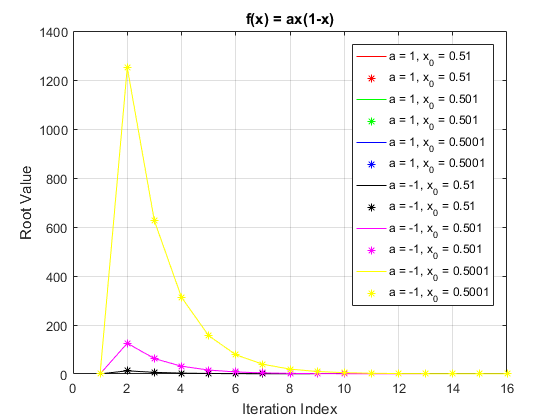
\includegraphics[scale=0.7]{q3_2.png}
    \caption{Positive root of $f(x) = ax(1-x)$}
\end{figure}
\newpage
\subsubsection{Tables}


\begin{table}[!ht]
\centering{\Large
\begin{tabular}{|c|c|c|c|c|c|}\hline
ItrNo   & $x_n$    & $f(x_n)$      & $f'(x_n)$      & $x_{n+1}$    & $x_{n+1}-x_n$ \\ \hline
1 & 0.51   & 0.2499  & -0.02   & 13.005 & 12.495  \\
2 & 13.005 & -156.13 & -25.01  & 6.7625 & -6.2425 \\
3 & 6.7625 & -38.969 & -12.525 & 3.6512 & -3.1113 \\
4 & 3.6512 & -9.6801 & -6.3024 & 2.1153 & -1.5359 \\
5 & 2.1153 & -2.3591 & -3.2305 & 1.385  & -0.7302 \\
6 & 1.385  & -0.5333 & -1.77   & 1.0838 & -0.3013 \\
7 & 1.0838 & -0.0908 & -1.1675 & 1.006  & -0.0777 \\
8 & 1.006  & -0.006  & -1.012  & 1      & -0.006  \\
9 & 1      & 0       & -1.0001 & 1      & 0       \\
\hline
\end{tabular}}
\caption{Root of $f(x) = ax(1-x)$ where $a = 1$ and Initial Point = $0.51$}
\end{table}
\begin{table}[!ht]
\centering{\Large
\begin{tabular}{|c|c|c|c|c|c|}\hline
ItrNo   & $x_n$    & $f(x_n)$      & $f'(x_n)$      & $x_{n+1}$    & $x_{n+1}-x_n$ \\ \hline
1  & 0.501  & 0.25    & -0.002  & 125.5  & 125     \\
2  & 125.5  & -15625  & -250    & 63.001 & -62.499 \\
3  & 63.001 & -3906.2 & -125    & 31.753 & -31.249 \\
4  & 31.753 & -976.48 & -62.505 & 16.13  & -15.622 \\
5  & 16.13  & -244.06 & -31.261 & 8.3232 & -7.8072 \\
6  & 8.3232 & -60.952 & -15.646 & 4.4276 & -3.8956 \\
7  & 4.4276 & -15.176 & -7.8551 & 2.4956 & -1.932  \\
8  & 2.4956 & -3.7324 & -3.9912 & 1.5604 & -0.9352 \\
9  & 1.5604 & -0.8745 & -2.1209 & 1.1481 & -0.4123 \\
10 & 1.1481 & -0.17   & -1.2962 & 1.0169 & -0.1312 \\
11 & 1.0169 & -0.0172 & -1.0338 & 1.0003 & -0.0166 \\
12 & 1.0003 & -0.0003 & -1.0006 & 1      & -0.0003 \\
13 & 1      & 0       & -1      & 1      & 0       \\
\hline
\end{tabular}}
\caption{Root of $f(x) = ax(1-x)$ where $a = 1$ and Initial Point = $0.501$}
\end{table}
\newpage
\begin{table}[!ht]
\centering{\Large
\begin{tabular}{|c|c|c|c|c|c|}\hline
ItrNo   & $x_n$    & $f(x_n)$      & $f'(x_n)$      & $x_{n+1}$    & $x_{n+1}-x_n$ \\ \hline
1  & 0.5001 & 0.25        & -0.0002 & 1250.5 & 1250    \\
2  & 1250.5 & -1.5625e+06 & -2500   & 625.5  & -625    \\
3  & 625.5  & -3.9062e+05 & -1250   & 313    & -312.5  \\
4  & 313    & -97656      & -625    & 156.75 & -156.25 \\
5  & 156.75 & -24414      & -312.5  & 78.626 & -78.124 \\
6  & 78.626 & -6103.4     & -156.25 & 39.565 & -39.061 \\
7  & 39.565 & -1525.8     & -78.129 & 20.035 & -19.529 \\
8  & 20.035 & -381.39     & -39.071 & 10.274 & -9.7614 \\
9  & 10.274 & -95.284     & -19.548 & 5.3999 & -4.8743 \\
10 & 5.3999 & -23.759     & -9.7997 & 2.9754 & -2.4244 \\
11 & 2.9754 & -5.8778     & -4.9509 & 1.7882 & -1.1872 \\
12 & 1.7882 & -1.4095     & -2.5764 & 1.2411 & -0.5471 \\
13 & 1.2411 & -0.2993     & -1.4823 & 1.0392 & -0.2019 \\
14 & 1.0392 & -0.0408     & -1.0785 & 1.0014 & -0.0378 \\
15 & 1.0014 & -0.0014     & -1.0029 & 1      & -0.0014 \\
16 & 1      & 0           & -1      & 1      & 0 \\
\hline
\end{tabular}}
\caption{Root of $f(x) = ax(1-x)$ where $a = 1$ and Initial Point = $0.5001$}
\end{table}
\begin{table}[!ht]
\centering{\Large
\begin{tabular}{|c|c|c|c|c|c|}\hline
ItrNo   & $x_n$    & $f(x_n)$      & $f'(x_n)$      & $x_{n+1}$    & $x_{n+1}-x_n$ \\ \hline
1 & 0.51   & -0.2499 & 0.02   & 13.005 & 12.495  \\
2 & 13.005 & 156.13  & 25.01  & 6.7625 & -6.2425 \\
3 & 6.7625 & 38.969  & 12.525 & 3.6512 & -3.1113 \\
4 & 3.6512 & 9.6801  & 6.3024 & 2.1153 & -1.5359 \\
5 & 2.1153 & 2.3591  & 3.2305 & 1.385  & -0.7302 \\
6 & 1.385  & 0.5333  & 1.77   & 1.0838 & -0.3013 \\
7 & 1.0838 & 0.0908  & 1.1675 & 1.006  & -0.0777 \\
8 & 1.006  & 0.006   & 1.012  & 1      & -0.006  \\
9 & 1      & 0       & 1.0001 & 1      & 0       \\
\hline
\end{tabular}}
\caption{Root of $f(x) = ax(1-x)$ where $a = -1$ and Initial Point = $0.51$}
\end{table}
\newpage
\begin{table}[!h]
\centering{\Large
\begin{tabular}{|c|c|c|c|c|c|}\hline
ItrNo   & $x_n$    & $f(x_n)$      & $f'(x_n)$      & $x_{n+1}$    & $x_{n+1}-x_n$ \\ \hline
1  & 0.501  & -0.25  & 0.002  & 125.5  & 125     \\
2  & 125.5  & 15625  & 250    & 63.001 & -62.499 \\
3  & 63.001 & 3906.2 & 125    & 31.753 & -31.249 \\
4  & 31.753 & 976.48 & 62.505 & 16.13  & -15.622 \\
5  & 16.13  & 244.06 & 31.261 & 8.3232 & -7.8072 \\
6  & 8.3232 & 60.952 & 15.646 & 4.4276 & -3.8956 \\
7  & 4.4276 & 15.176 & 7.8551 & 2.4956 & -1.932  \\
8  & 2.4956 & 3.7324 & 3.9912 & 1.5604 & -0.9352 \\
9  & 1.5604 & 0.8745 & 2.1209 & 1.1481 & -0.4123 \\
10 & 1.1481 & 0.17   & 1.2962 & 1.0169 & -0.1312 \\
11 & 1.0169 & 0.0172 & 1.0338 & 1.0003 & -0.0166 \\
12 & 1.0003 & 0.0003 & 1.0006 & 1      & -0.0003 \\
13 & 1      & 0      & 1      & 1      & 0       \\
\hline
\end{tabular}}
\caption{Root of $f(x) = ax(1-x)$ where $a = -1$ and Initial Point = $0.501$}
\end{table}

\begin{table}[!h]
\centering{\Large
\begin{tabular}{|c|c|c|c|c|c|}\hline
ItrNo   & $x_n$    & $f(x_n)$      & $f'(x_n)$      & $x_{n+1}$    & $x_{n+1}-x_n$ \\ \hline
1  & 0.5001 & -0.25      & 0.0002 & 1250.5 & 1250    \\
2  & 1250.5 & 1.5625e+06 & 2500   & 625.5  & -625    \\
3  & 625.5  & 3.9062e+05 & 1250   & 313    & -312.5  \\
4  & 313    & 97656      & 625    & 156.75 & -156.25 \\
5  & 156.75 & 24414      & 312.5  & 78.626 & -78.124 \\
6  & 78.626 & 6103.4     & 156.25 & 39.565 & -39.061 \\
7  & 39.565 & 1525.8     & 78.129 & 20.035 & -19.529 \\
8  & 20.035 & 381.39     & 39.071 & 10.274 & -9.7614 \\
9  & 10.274 & 95.284     & 19.548 & 5.3999 & -4.8743 \\
10 & 5.3999 & 23.759     & 9.7997 & 2.9754 & -2.4244 \\
11 & 2.9754 & 5.8778     & 4.9509 & 1.7882 & -1.1872 \\
12 & 1.7882 & 1.4095     & 2.5764 & 1.2411 & -0.5471 \\
13 & 1.2411 & 0.2993     & 1.4823 & 1.0392 & -0.2019 \\
14 & 1.0392 & 0.0408     & 1.0785 & 1.0014 & -0.0378 \\
15 & 1.0014 & 0.0014     & 1.0029 & 1      & -0.0014 \\
16 & 1      & 0          & 1      & 1      & 0 \\
\hline
\end{tabular}}
\caption{Root of $f(x) = ax(1-x)$ where $a = -1$ and Initial Point = $0.5001$}
\end{table}


\newpage
\section{$f(x) = a + x(x-1)^2$}
\subsection{Different Initial Points for $a = 0$}
\begin{figure}[!h]
    \centering
    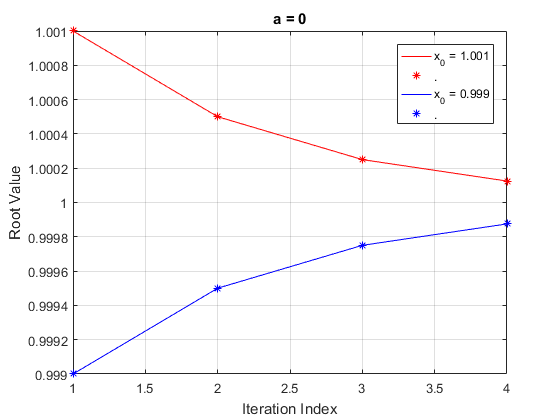
\includegraphics[scale=0.8]{q4_1.png}
    \caption{Positive root of $f(x) = ax(1-x)$}
\end{figure}
\begin{table}[!h]
\centering{\Large
\begin{tabular}{|c|c|c|c|c|c|}\hline
ItrNo   & $x_n$    & $f(x_n)$      & $f'(x_n)$      & $x_{n+1}$    & $x_{n+1}-x_n$ \\ \hline
1 & 0.999  & 0 & -0.002  & 0.9995 & 0.0005 \\
2 & 0.9995 & 0 & -0.001  & 0.9998 & 0.0002 \\
3 & 0.9998 & 0 & -0.0005 & 0.9999 & 0.0001 \\
4 & 0.9999 & 0 & -0.0002 & 0.9999 & 0.0001 \\
\hline
\end{tabular}}
\caption{Root of $f(x) = a + x(x-1)^2$ where $a = 0$ and Initial Point = $0.999$}
\end{table}

\begin{table}[!h]
\centering{\Large
\begin{tabular}{|c|c|c|c|c|c|}\hline
ItrNo   & $x_n$    & $f(x_n)$      & $f'(x_n)$      & $x_{n+1}$    & $x_{n+1}-x_n$ \\ \hline
1 & 1.001  & 0 & 0.002   & 1.0005 & -0.0005 \\
2 & 1.0005 & 0 & 0.001   & 1.0003 & -0.0003 \\
3 & 1.0003 & 0 & 0.0005  & 1.0001 & -0.0001 \\
4 & 1.0001 & 0 & 0.0003  & 1.0001 & -0.0001 \\
\hline
\end{tabular}}
\caption{Root of $f(x) = a + x(x-1)^2$ where $a = 0$ and Initial Point = $1.001$}
\end{table}
\newpage
\subsection{Different Initial Points for $a = 0.03$}
\begin{table}[!h]
\centering{\Large
\begin{tabular}{|c|c|c|c|c|c|}\hline
ItrNo   & $x_n$    & $f(x_n)$      & $f'(x_n)$      & $x_{n+1}$    & $x_{n+1}-x_n$ \\ \hline
1  & 0.999   & 0.03    & -0.002  & 16.022  & 15.023  \\
2  & 16.022  & 3615.6  & 707.03  & 10.908  & -5.1138 \\
3  & 10.908  & 1070.9  & 314.34  & 7.5013  & -3.407  \\
4  & 7.5013  & 317.09  & 139.8   & 5.2332  & -2.2681 \\
5  & 5.2332  & 93.81   & 62.227  & 3.7257  & -1.5075 \\
6  & 3.7257  & 27.709  & 27.739  & 2.7268  & -0.9989 \\
7  & 2.7268  & 8.1603  & 12.399  & 2.0686  & -0.6582 \\
8  & 2.0686  & 2.3921  & 5.5628  & 1.6386  & -0.43   \\
9  & 1.6386  & 0.6982  & 2.5005  & 1.3594  & -0.2792 \\
10 & 1.3594  & 0.2055  & 1.1061  & 1.1735  & -0.1858 \\
11 & 1.1735  & 0.0653  & 0.4374  & 1.0242  & -0.1494 \\
12 & 1.0242  & 0.0306  & 0.0501  & 0.413   & -0.6112 \\
13 & 0.413   & 0.1723  & -0.1403 & 1.6415  & 1.2285  \\
14 & 1.6415  & 0.7055  & 2.5175  & 1.3613  & -0.2802 \\
15 & 1.3613  & 0.2076  & 1.114   & 1.1749  & -0.1864 \\
16 & 1.1749  & 0.0659  & 0.4414  & 1.0255  & -0.1493 \\
17 & 1.0255  & 0.0307  & 0.053   & 0.4469  & -0.5786 \\
18 & 0.4469  & 0.1667  & -0.1884 & 1.3318  & 0.8849  \\
19 & 1.3318  & 0.1766  & 0.9937  & 1.1541  & -0.1777 \\
20 & 1.1541  & 0.0574  & 0.3793  & 1.0028  & -0.1513 \\
21 & 1.0028  & 0.03    & 0.0055  & -4.416  & -5.4187 \\
22 & -4.416  & -129.5  & 77.167  & -2.7378 & 1.6782  \\
23 & -2.7378 & -38.219 & 34.437  & -1.6279 & 1.1098  \\
24 & -1.6279 & -11.213 & 15.462  & -0.9028 & 0.7252  \\
25 & -0.9028 & -3.2386 & 7.0562  & -0.4438 & 0.459   \\
26 & -0.4438 & -0.8952 & 3.3661  & -0.1779 & 0.2659  \\
27 & -0.1779 & -0.2168 & 1.8064  & -0.0579 & 0.12    \\
28 & -0.0579 & -0.0348 & 1.2415  & -0.0299 & 0.028   \\
29 & -0.0299 & -0.0017 & 1.1222  & -0.0284 & 0.0015  \\
30 & -0.0284 & 0       & 1.1159  & -0.0284 & 0 \\
\hline
\end{tabular}}
\caption{Root of $f(x) = a + x(x-1)^2$ where $a = 0.03$ and Initial Point = $0.999$}
\end{table}

\begin{table}[!h]
\centering{\Large
\begin{tabular}{|c|c|c|c|c|c|}\hline
ItrNo   & $x_n$    & $f(x_n)$      & $f'(x_n)$      & $x_{n+1}$    & $x_{n+1}-x_n$ \\ \hline
1  & 1.001   & 0.03    & 0.002  & -13.977 & -14.978 \\
2  & -13.977 & -3135.2 & 642.98 & -9.101  & 4.876   \\
3  & -9.101  & -928.55 & 285.89 & -5.8531 & 3.2479  \\
4  & -5.8531 & -274.86 & 127.19 & -3.692  & 2.161   \\
5  & -3.692  & -81.251 & 56.662 & -2.2581 & 1.434   \\
6  & -2.2581 & -23.939 & 25.329 & -1.3129 & 0.9451  \\
7  & -1.3129 & -6.9937 & 11.423 & -0.7007 & 0.6122  \\
8  & -0.7007 & -1.9966 & 5.2756 & -0.3222 & 0.3785  \\
9  & -0.3222 & -0.5333 & 2.6004 & -0.1171 & 0.2051  \\
10 & -0.1171 & -0.1162 & 1.5097 & -0.0402 & 0.077   \\
11 & -0.0402 & -0.0135 & 1.1655 & -0.0286 & 0.0116  \\
12 & -0.0286 & -0.0003 & 1.1169 & -0.0284 & 0.0003  \\
13 & -0.0284 & 0       & 1.1159 & -0.0284 & 0       \\
\hline
\end{tabular}}
\caption{Root of $f(x) = a + x(x-1)^2$ where $a = 0.03$ and Initial Point = $1.001$}
\end{table}

\begin{figure}[!h]
    \centering
    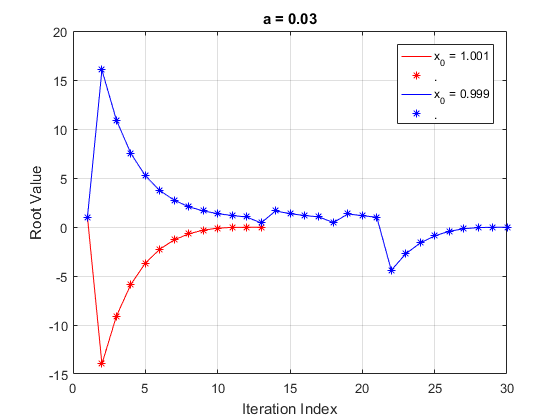
\includegraphics[scale=0.8]{q4_2.png}
    \caption{Positive root of $f(x) = ax(1-x)$}
\end{figure}
\newpage
\subsection{Different Initial Points for $a = 0.07$}
\begin{table}[!h]
\centering{\Large
\begin{tabular}{|c|c|c|c|c|c|}\hline
ItrNo   & $x_n$    & $f(x_n)$      & $f'(x_n)$      & $x_{n+1}$    & $x_{n+1}-x_n$ \\ \hline
1  & 0.999   & 0.07    & -0.002  & 36.052  & 35.053  \\
2  & 36.052  & 44295   & 3756    & 24.259  & -11.793 \\
3  & 24.259  & 13124   & 1669.5  & 16.398  & -7.8611 \\
4  & 16.398  & 3888    & 742.09  & 11.159  & -5.2392 \\
5  & 11.159  & 1151.6  & 329.91  & 7.668   & -3.4907 \\
6  & 7.668   & 341     & 146.72  & 5.3438  & -2.3242 \\
7  & 5.3438  & 100.9   & 65.294  & 3.7985  & -1.5453 \\
8  & 3.7985  & 29.818  & 29.092  & 2.7735  & -1.025  \\
9  & 2.7735  & 8.7938  & 12.983  & 2.0962  & -0.6773 \\
10 & 2.0962  & 2.5889  & 5.7974  & 1.6496  & -0.4466 \\
11 & 1.6496  & 0.7662  & 2.5653  & 1.351   & -0.2987 \\
12 & 1.351   & 0.2364  & 1.0715  & 1.1303  & -0.2206 \\
13 & 1.1303  & 0.0892  & 0.3116  & 0.8441  & -0.2863 \\
14 & 0.8441  & 0.0905  & -0.2389 & 1.223   & 0.3789  \\
15 & 1.223   & 0.1308  & 0.595   & 1.0032  & -0.2198 \\
16 & 1.0032  & 0.07    & 0.0063  & -10.043 & -11.046 \\
17 & -10.043 & -1224.5 & 343.73  & -6.4802 & 3.5624  \\
18 & -6.4802 & -362.51 & 152.9   & -4.1092 & 2.3709  \\
19 & -4.1092 & -107.2  & 68.094  & -2.535  & 1.5743  \\
20 & -2.535  & -31.607 & 30.418  & -1.4959 & 1.0391  \\
21 & -1.4959 & -9.2484 & 13.696  & -0.8206 & 0.6752  \\
22 & -0.8206 & -2.6502 & 6.3028  & -0.4002 & 0.4205  \\
23 & -0.4002 & -0.7145 & 3.081   & -0.1683 & 0.2319  \\
24 & -0.1683 & -0.1596 & 1.758   & -0.0774 & 0.0908  \\
25 & -0.0774 & -0.0199 & 1.3278  & -0.0625 & 0.015   \\
26 & -0.0625 & -0.0005 & 1.2615  & -0.0621 & 0.0004  \\
27 & -0.0621 & 0       & 1.2598  & -0.0621 & 0       \\
\hline
\end{tabular}}
\caption{Root of $f(x) = a + x(x-1)^2$ where $a = 0.07$ and Initial Point = $0.999$}
\end{table}
\begin{figure}[!h]
    \centering
    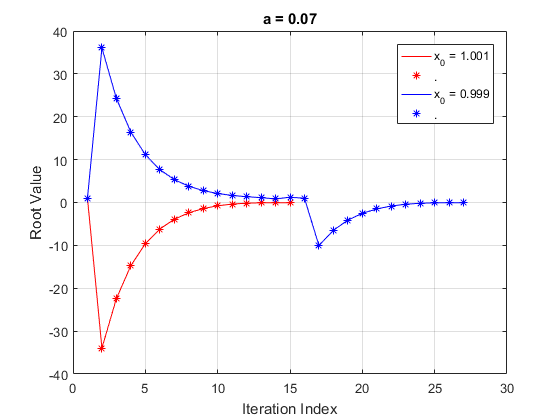
\includegraphics[scale=0.8]{q4_3.png}
    \caption{Positive root of $f(x) = ax(1-x)$}
\end{figure}
\begin{table}[!h]
\centering{\Large
\begin{tabular}{|c|c|c|c|c|c|}\hline
ItrNo   & $x_n$    & $f(x_n)$      & $f'(x_n)$      & $x_{n+1}$    & $x_{n+1}-x_n$ \\ \hline
1  & 1.001   & 0.07    & 0.002  & -33.947 & -34.948 \\
2  & -33.947 & -41459  & 3594   & -22.411 & 11.536  \\
3  & -22.411 & -12283  & 1597.5 & -14.722 & 7.6894  \\
4  & -14.722 & -3638.9 & 710.1  & -9.5974 & 5.1245  \\
5  & -9.5974 & -1077.8 & 315.72 & -6.1838 & 3.4137  \\
6  & -6.1838 & -319.05 & 140.45 & -3.9121 & 2.2716  \\
7  & -3.9121 & -94.327 & 62.563 & -2.4044 & 1.5077  \\
8  & -2.4044 & -27.798 & 27.962 & -1.4103 & 0.9941  \\
9  & -1.4103 & -8.1232 & 12.608 & -0.766  & 0.6443  \\
10 & -0.766  & -2.319  & 5.8244 & -0.3679 & 0.3982  \\
11 & -0.3679 & -0.6183 & 2.8773 & -0.153  & 0.2149  \\
12 & -0.153  & -0.1334 & 1.6821 & -0.0737 & 0.0793  \\
13 & -0.0737 & -0.015  & 1.3111 & -0.0623 & 0.0114  \\
14 & -0.0623 & -0.0003 & 1.2608 & -0.0621 & 0.0002  \\
15 & -0.0621 & 0       & 1.2598 & -0.0621 & 0       \\
\hline
\end{tabular}}
\caption{Root of $f(x) = a + x(x-1)^2$ where $a = 0.07$ and Initial Point = $1.001$}
\end{table}




\end{document}